\section{\texorpdfstring{Silne regulární grafy, propletani vl cisel}{Silne regulární grafy, propletani vl cisel}}
\vspace{5mm}
\large

\begin{definition}
	Silně regulární je graf pokud není uplný (triviální případ) a $\exists d,e,f \in \N: \forall v \in V \ deg(v) = d$.
	Každé 2 sousední vrcholy mají $e$ společných sousedu (2 vrcholy leží v $e \triangle$), každé 2 nesousední vrcholy mají $f$ společných sousedu ($\exists f$ cest délky 2).
\end{definition}

\begin{theorem}[Silne regulární grafy (nebude u zkousky)]
	Je-li $G$ silné regulární s parametry $d,e,f$, pak nastává jedna z 2 možností:
	\begin{itemize}
		\item $f = e + 1, d = 2f, |V(G)| = 2d + 1$ nebo
		\item $\exists s \in \N: s^2 = (e - f)^2 - 4(f - d) \land \frac{d}{2fs}((d - 1 + f - e)(s + f - e) - 2f) \in \N$.
	\end{itemize}
\end{theorem}
\begin{proof}
	Nechť A je matice sousednosti G, $n = |V(G)|$, uvažme $A^2$.
	Na diagonále jsou stupně $d$, mimo diagonálu pokud v A byla 1 - změní se na $e$, 0 se změní na $f$.

	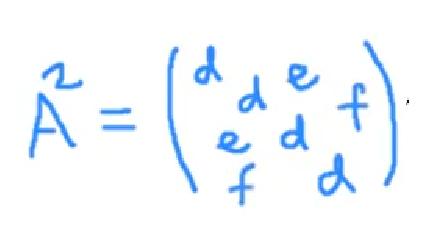
\includegraphics[scale=0.5]{s_reg_1.eps}

	\[ A^2 = dI + eA + (J -I - A)f \Rightarrow A^2 + (f - e)A + (f - d)I = fJ \]
	Dosadíme vlastní číslo $\lambda \in Sp(A)$.
	\[ \lambda^2 + (f - e)\lambda + (f - d) \in Sp(fJ) = \{ f * n, 0^{(n-1)} \} \]

	$d$ odpovídá vlastnímu vektoru $\bar{1}$ u A, u J vlastnímu vektoru $\bar{1}$ odpovídá $n$. Dosadíme $d$:
	\[ d^2 + (f - e)d + f - d = fn \Rightarrow d(d - e - 1) = f(n - d - 1)\]

	Zafixujme nějaký vrchol $x \in V$. Kolik $\exists$ indukovaných cest délky 2:
	\[ |\{ (x,a) | xa, ab \in E(G) \land xb \notin E(g) \}| \]

	Máme $d$ způsobu zvolit souseda $x$, pak vrchol $a$ má $d$ sousedu, $e$ jsou společné s $x$, $x$ taky patří mezi sousedy. Dostaneme $d (d - e - 1)$.
	Na druhou stranu z pohledu vrcholu $b$. $X$ má $(n - d - 1)$ nesousedu, pak vrchol $a$ je mezi $f$ sousedu $(x,b)$. Dostaneme $f(n - d - 1)$.

	Pro $\lambda \in Sp(A)\setminus \{d\}$ zbývá 0:
	\[ \lambda^2 + (f - e)\lambda + f - d = 0 \Rightarrow \lambda_{1,2} = \frac{e - f \pm \sqrt{(e - f)^2 - 4 (f - d)}}{2} \]
	Označme $D = \sqrt{(e - f)^2 - 4 (f - d)}$. Pak $\lambda_1 = 1/2 (e - f + s), p$ krát a $\lambda_2 = 1/2 (e - f - s), q$ krát.

	Z násobnosti vlastních čísel
	\begin{equation*}
	\begin{aligned}
	 1 + p + q = n \\
	 a + p\lambda_1 + q \lambda_2 = tr(A) = 0 \\
	 tr(A^2) = \sum \lambda_i^2 = nd \Rightarrow d^2 + p \lambda_1^2 + q \lambda_2^2 = nd
	\end{aligned}
	\end{equation*}

	Vyřešíme soustavu 3 rovnic o 3 neznámých.
	Dosadíme hodnoty $\lambda_1, \lambda_2$ do 2. rovnice:
	\[ d + 1/2 p (e - d + s) + 1/2 q (e - f - s) = 0 \Rightarrow d + 1/2(p + q) (e - f) + 1/2 (p - q) s = 0 \]

	Nastávaji 2 případy:\\
	1) $s \notin \Q \Rightarrow$ poslední sčítanec je iracionální a nutně $ p = q = 1/2 (n - 1)$.
	\[ d + 1/2 (n-1) (e - f) = 0 \Rightarrow \frac{2d}{n - 1} = (f - e) \]
	Pak stupeň vrcholu $ d \leq (n - 1)$
	\[ \frac{2d}{n - 1} = (f - e) \leq \frac{2 (n-1)}{2} = 2 \]
	Pokud $(f - e) = 2 \Rightarrow d = n-1 \Rightarrow G = K_n$ což jsme vyloučili definici. Jinak
	\[(f - e) = 1 \land n = 2d + 1 \]
	Pracujme s 3. rovnici:
	\[ d^2 + 1/2 (n-1) * 1/4 (e - f + s)^2 + 1/2 (n-1) * 1/4 (e - f -s)^2 = nd \]
	dosadíme $(e - f) = -1$.
	\begin{equation*}
	\begin{aligned}
	 d^2 + 1/2 (n-1) * 1/4 (s - 1)^2 + 1/2 (n-1) * 1/4 (-1 - s)^2 = nd \\
	 8d^2 + (n-1)(s^2 - 2s + 1) + (n-1)(s^2 + 2s + 1) = 8nd \\
	 8d^2 + (n-1)(s^2 - 2s + 1 + s^2 + 2s + 1) = 8nd \\
	 8d^2 + (n-1)(2s^2 + 2) = 8nd \\
	 4d^2 + (n-1)(s^2 + 1) = 4nd
	\end{aligned}
	\end{equation*}
	Dosadíme $n = 2d - 1$
	\[ 4d^2 + 2d(s^2 + 1) = 4(2d + 1)d \]
	\[ 2d + (s^2 + 1) = 2(2d + 1) \]
	Pak $s^2 = 1 + 4(d - f)$
	\[ 2d + 2 + 4d - 4f = 4d + 2 \]
	\[ 2d = 4f \Rightarrow d = 2f \]
	2) Jinak $s \in \Z$ dosadíme do 2. a 3. rovnice $n$, vyřešíme pro $p,q$.
	\begin{equation*}
	\begin{aligned}
		d + 1/2 p (e - d + s) + 1/2 q (e - f - s) = 0 \\
		d^2 + 1/2 (n-1) * 1/4 (e - f + s)^2 + 1/2 (n-1) * 1/4 (e - f -s)^2 = (1 + q + p)d \\
	\end{aligned}
	\end{equation*}
	Zbavíme se jmenovatele a roznásobíme kvadráty v 3.
	\begin{equation*}
	\begin{aligned}
		p (e - d + s) + 1/2 q (e - f - s) = 2d \\
		p((e - f + s)^2 - 4d) + q((e - f -s)^2 - 4d) = 4d (1 - d)
	\end{aligned}
	\end{equation*}
	Spočítáme $p,q$ pomoci determinantu.

	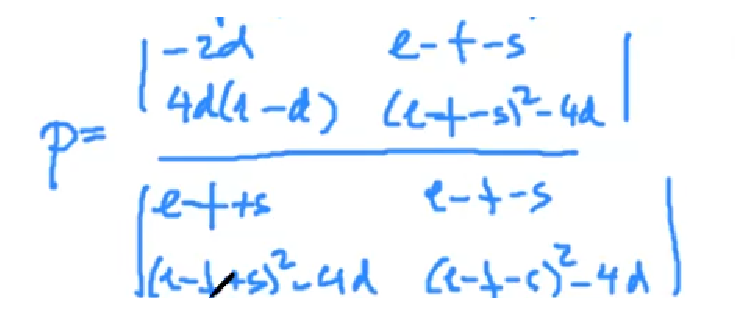
\includegraphics[scale=0.5]{s_reg_2.eps}

	Dolní determinant
	\begin{equation*}
	\begin{split}
		(e - f + s)((e - f - s)^2 -4d) - (e - f - s)((e - f + s)^2 - 4d) = \\
		(e - f + s)(e - f - s)(e - f -s - e + f - s) + 4d (e + f - s + e - f - s) = \\
		((e - f)^2 - s^2)(-2s) + 4d (-2s) = (-2s)((e - f)^2 + 4d - s^2)
	\end{split}
	\end{equation*}
	Dosadíme $s^2 = (e - f)^2 + 4(d - f)$.
	\[ (-2s)((e - f)^2 + 4d - (e - f)^2 + 4(d - f)) = -8fs \]

	Horní determinant:

	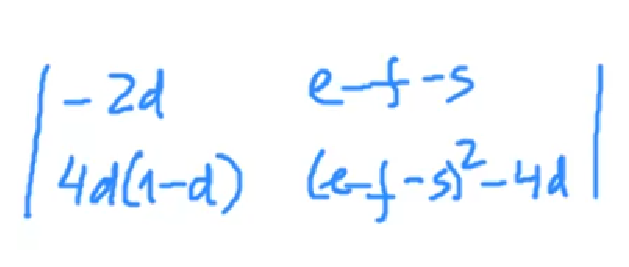
\includegraphics[scale=0.5]{s_reg_3.eps}

	2 hours later...
	\[ p = \frac{d((d - 1 + f - e)(s + f - e) - 2f)}{2fs} \in \Z \]
\end{proof}

\begin{theorem}[Friendship theorem]
	Nechť v grafu $G$ mají každé 2 různé vrcholy právě 1 společného souseda.
	Pak $G$ obsahuje vrchol, který sousedi se všemi ostatní vrcholy grafu.
\end{theorem}
\begin{proof}
	Pokud platí $ e = f = 1 \Rightarrow \exists v \in V$ který sousedi se všemi ostatní vrcholy. \\
	Nechť $N_G(u)$ je množina sousedu $u \in V$. Vezmeme množinový systém $\{ N_G(u) | u \in V \}$.

	Pak průnik dvou množin je jednoprvkový.
	\[ \forall a \ne b: |N_G(a) \cap N_G(b)| = 1 \]
	Taky z obrázku

	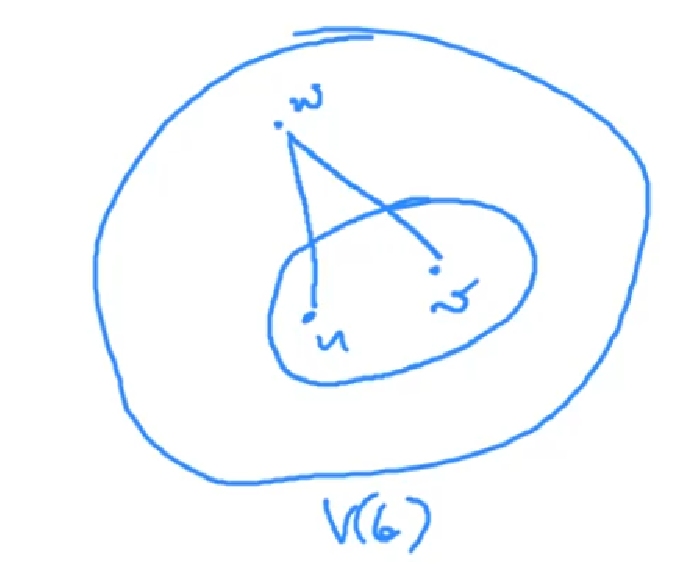
\includegraphics[scale=0.5]{fiendship_1.eps}

	\[ \forall a \ne b\ \exists! N_G(w): a,b \in N_G(w) \]
	Což je skoro konečná projektivní rovina KPR. Chybí 3. axiom. Rozebereme 2 případy:

	1) 3. axiom platí $\Rightarrow \{N_G\}$ je KPR. Pak
	\begin{equation*}
	\begin{split}
		\forall a |N_G(a)| = m + 1 = deg(a) \\
		n = |V(G)| = m^2 + m + 1\\
	\end{split}
	\end{equation*}
	Z čehož $G$ je silné regulární s parametry $ d = m + 1 \land e = f = 1$. První případ nastat nemůže kvůli podmínce na $e = f = 1$. Neboli 2 případ:

	\begin{equation*}
	\begin{aligned}
		p = \frac{d((d - 1 + f - e)(s + f - e) - 2f)}{2fs} \in \Z \\
		(e - f)^2 - 4 (f - d) = s^2 \land e = f = 1 \Rightarrow s = 2 \sqrt{m} = 2t
	\end{aligned}
	\end{equation*}
	Dosadíme
	\[ p = \frac{t^2 + 1}{4t}((t^2 * 2t) - 2) = \frac{(t^2 + 1)(t^3 - 1)}{2t} \notin N : t > 1 \]
	Případ $t = 1 \Rightarrow m = 1$ není zajímavý protože KPR radu 1 je $\triangle$.

	2) 3. axiom neplatí $\Rightarrow \{N_G\}$ z teorie KPR bud všechno leží na 1 přímce nebo jeden vrchol samostatně a zbytek na přímce. Pak ten samostatný vrchol je hledaný soused všech:
	\[ \exists a : N_G(a) = V(G)\setminus \{a\} \]

\end{proof}
\begin{theorem}[vl čísla Hermitovske matice(BD)]
	Nechť $A \in \Comp^{n \times n}$ je Hermitovska, $\lambda_1 \geq \lambda_2 \geq ... \geq \lambda_n$ její vlastní čísla.
	Nechť $b_1, b_2, ..., b_n \in \Comp^n$ je ortonormální báze z vlastních vektoru. Pak pro $k = 1, 2, ..., n$ platí
	\[ x^{\ast}Ax \geq \lambda_k x^{\ast}x \forall x \in \langle \{ b_1, b_2, ..., b_k\} \rangle \]
	\[ x^{\ast}Ax \leq \lambda_k x^{\ast}x \forall x \in \langle \{ b_k, b_{k+1}, ..., b_n\} \rangle \]
\end{theorem}

\begin{theorem}[Propletani vl cisel]
	Nechť $A \in \Comp^{n \times n}$ je Hermitovska, $\lambda_1 \geq \lambda_2 \geq ... \geq \lambda_n$ její vlastní čísla.
	Nechť $B$ je hlavni podmatice radu $k \times k$ (vznikne vynecháním $(n - k)$ řádky),
	Nechť $b_1, b_2, ..., b_n \in \Comp^n$ jsou vlastní čísla matice $B$. Pak platí
	\[ \lambda_i \geq b_i \geq \lambda_{i + n - k} \]
\end{theorem}
\begin{proof}
	Nejprve se podíváme na případ vynechaní i-ho řádku.
	Nechť $B$ má ortonormální báze $y_1, y_2, ..., y_{n-1} \in \Comp^{n - 1}$.
	Vnoříme tyto vektory do $\Comp^n$ tak, ze na pozici $i - 1$ vložíme 0.
	Označíme je $z(y)$.
	Pak
	\[ z^{\ast}(y)Az(y) = y^{\ast}By \]
	Uvažme 3 množiny, $j$ je libovolné
	\begin{gather*}
		S_1 = \langle\{x_j, x_{j+1},..., x_n\} \rangle \\
		S_2 = \langle\{y_1, y_2,..., y_j\} \rangle \\
		S_3 = \{z(y): y \in S_2 \} \\
		dim S_1 = n - j + 1 \\
		dim S_3 = dim S_2 = j \\
		dim S_1 + dim S_3 = n+1 > dim (S_1 + S_2)
	\end{gather*}
	Z toho $dim(S_1 \cap S_2) > 0 \Rightarrow \exists l \ne 0 : l \in S_1 \cap S_2$.
	Podíváme se na
	\begin{gather*}
		l \in S_1 \Rightarrow l^{\ast}Al \geq \lambda_j l^{\ast}l \\
		l \in S_3, y \in S_2, l = z(y): l^{\ast}Al = y^{\ast}By \geq b_j y y^{\ast} = b_j l^{\ast} l \leq \lambda_j l^{\ast}l \\
		\lambda_j l^{\ast}l \geq b_j l^{\ast}l\ \Rightarrow \lambda_j \geq b_j
	\end{gather*}

	Teď dokážeme $ b_j \geq \lambda_{j + 1} $
	\begin{gather*}
		S_1 = \langle\{x_1, x_2,..., x_{j+1}\} \rangle \\
		S_2 = \langle\{y_j, y_{j+1},..., y_{n-1}\} \rangle \\
		S_3 = \{z(y): y \in S_2 \} \\
		dim S_1 = j + 1 \\
		dim S_3 = dim S_2 = n - j \\
		dim S_1 + dim S_3 = n+1 > dim (S_1 + S_2)
	\end{gather*}

	\begin{gather*}
		l \in S_1 \Rightarrow l^{\ast}Al \geq \lambda_{j + 1} l^{\ast}l \\
		l \in S_3, y \in S_2, l = z(y): l^{\ast}Al = y^{\ast}By \leq b_j y y^{\ast} = b_j l^{\ast} l \geq \lambda_{j + 1} l^{\ast}l \\
		\lambda_j l^{\ast}l \geq b_j l^{\ast}l\ \Rightarrow \lambda_{j + 1} \leq b_j
	\end{gather*}

	Teď pro obecně k.

	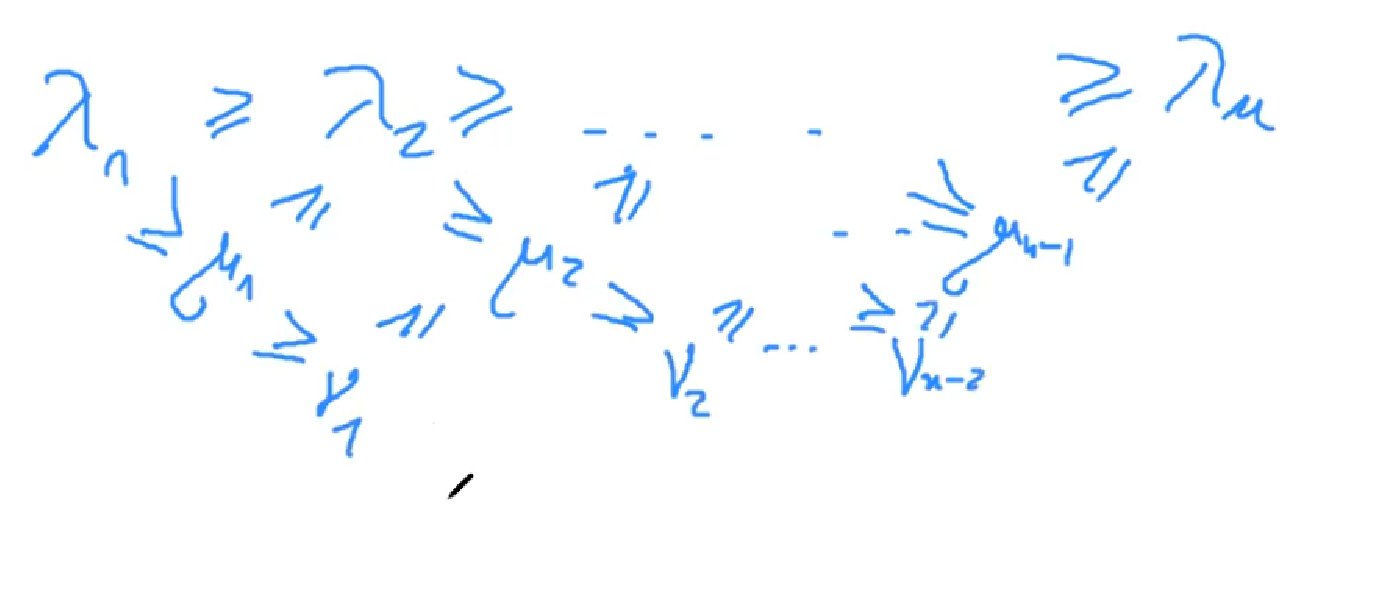
\includegraphics[scale=0.5]{eigen_prop.eps}

	Z obrázku
	\[ \lambda_i \geq k_i \geq \lambda_{i + k}, i = 1,2,..., n-k  \]

\end{proof}

\begin{theorem}[Nezav množina a vl čísla]
	Nechť $G$ je graf o $n$ vrcholech s vlastních čísly $\lambda_1 \geq \lambda_2 \geq ... \geq \lambda_n$. Pak
	\[ \alpha(G) \leq \min\{|\{i : \lambda_i \leq 0\}|, |\{i : \lambda_i \geq 0\}|\} \]
\end{theorem}
\begin{proof}
	Nechť $W \subseteq V(G)$ je nezávislá množina velkosti $\alpha$. Matice sousednosti teto množiny je nulová $\alpha \times \alpha$.
	Taky je to hlavní podmatice $A_G$. Proto její vlastní čísla (nuly) propletaji vlastní čísla $G$. Z toho
	\[ \lambda_{\alpha} \geq 0 \geq \lambda_{n - \alpha + 1} \]
\end{proof}
